\documentclass[10pt, compress]{beamer}

\usetheme{m}

\usepackage{booktabs}
\usepackage[scale=2]{ccicons}
\usepackage{minted}
% ---
% Graficos
% ---
\usepackage{tikz}
\usepackage{pgfplots}

\usemintedstyle{trac}

\definecolor{UBCblue}{rgb}{0.0, 0.0, 0.26667} % UBC Blue (primary)

\usecolortheme[named=UBCblue]{structure}

\title{ESP8266: Uma introdução ao IoT}
\subtitle{}
\date{\today}
\author{Gabriel Melo}
\institute{Emakers Júnior
\includegraphics[width=50pt]{images/emakersjr_logo.jpg}}
\begin{document}

\maketitle


\begin{frame}[fragile]
  \frametitle{mtheme}

  Este material é um resumo do livro homônimo, disponível em: \href{https://github.com/GabrielMMelo/esp8266\_course}{ \textit{ESP8266: Uma introdução ao IoT}
  } por Gabriel Melo.

\end{frame}

\begin{frame}[fragile]
  \frametitle{Sections}
  Sections group slides of the same topic

  \begin{minted}[fontsize=\small]{latex}
    \section{Elements}
  \end{minted}

\end{frame}

\section{Introdução}

\begin{frame}[fragile]
  \frametitle{Sinal Analógico}

  \begin{center}becomes\end{center}

  \begin{figure}[ht]
     \centering
    \label{Sinal-Analogico}
    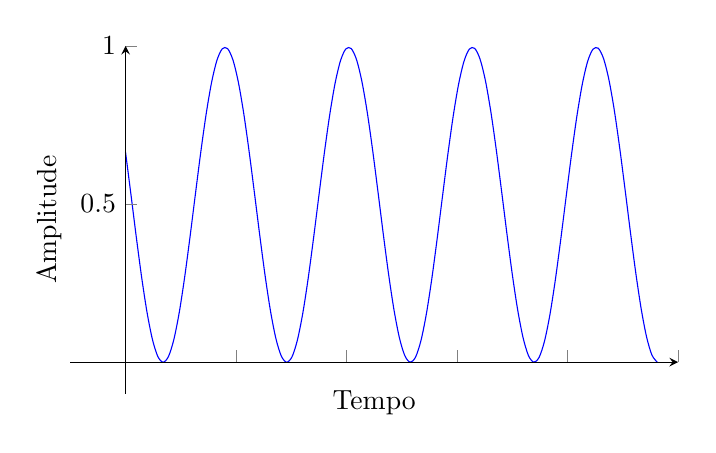
\begin{tikzpicture}
      %\draw[->] (-2,0) -- (5.3,0);
      %\draw[->] (-2,-2) -- (-2,2);
      {\draw[blue,smooth,samples=100,domain= 0.7:7.455]
      plot(\x,{2.4+2*sin(\x r*4 )});}
      \begin{axis}[
        width=9.3cm,
        height=6cm,
        x axis line style={-stealth},
        y axis line style={-stealth},
         % title={Square wave},
       xticklabels={},
       ymax = 1.2,xmax=7.5,
       axis lines*=center,
       ytick={0.5,1},
       xlabel={Tempo},
       ylabel={Amplitude},
       xlabel near ticks,
       ylabel near ticks]
     \end{axis}
   \end{tikzpicture}
   \caption{Sinal Analógico}   
  \end{figure}

\end{frame}


\begin{frame}[fragile]
\frametitle{Sinal digital}

\begin{center}becomes\end{center}

\begin{figure}[ht]
\centering
\label{Sinal-Digital}
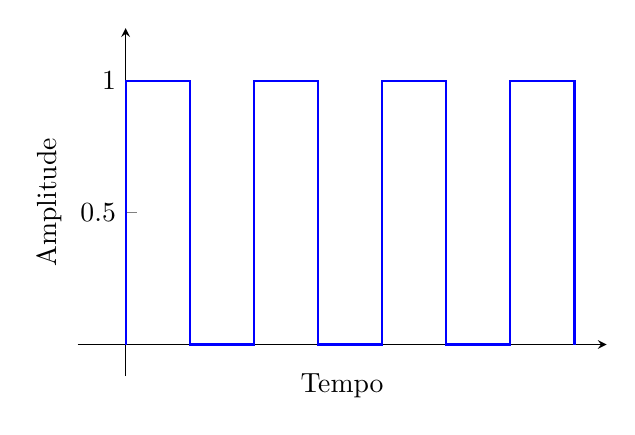
\begin{tikzpicture}
\begin{axis}[
width=8.3cm,
height=6cm,
      x axis line style={-stealth},
          y axis line style={-stealth},
             % title={Square wave},
             xticklabels={},
             ymax = 1.2,xmax=7.5,
             axis lines*=center,
             ytick={0.5,1},
             xlabel={Tempo},
             ylabel={Amplitude},
             xlabel near ticks,
             ylabel near ticks]
             \addplot+[thick,mark=none,const plot]
             coordinates
               {(0,0) (0,1) (1,0) (2,1) (3,0) (4,1) (5,0) (6,1) (7,0)};
         \end{axis}
     \end{tikzpicture}
     \caption{Sinal Digital}
  \end{figure}
\end{frame}

\begin{frame}{Descriptions}
\frametitle{Microcontrolador}
  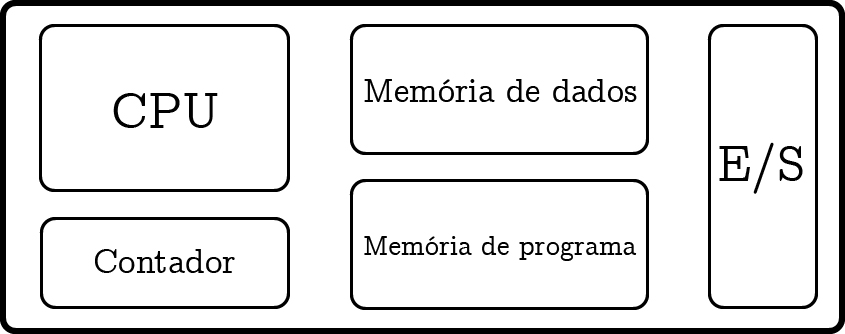
\includegraphics[width=30em]{images/Microcontrolador.jpg}
\end{frame}

\begin{frame}{Lists}
\frametitle{Memória}
\end{frame}

\begin{frame}{Figures}
  \frametitle{Wi-Fi}
  modos sta e ap (e o ap\_sta)
\end{frame}

\section{ESP8266}

\begin{frame}{Summary}
  \frametitle{O que é?}
\end{frame}

\begin{frame}{Modelos}
  \frametitle{Modelos}
\end{frame}

\begin{frame}{Animation}
  \frametitle{Especificações}
\end{frame}

\begin{frame}{Comunicação}
  \frametitle{Comunicação}
\end{frame}

\begin{frame}{SPIFFS}
  \frametitle{SPIFFS}
\end{frame}

\begin{frame}{Interrupção}
  \frametitle{Interrupção}
\end{frame}

\begin{frame}{Consumo de Energia}
  \frametitle{Consumo de Energia}
\end{frame}

\begin{frame}{Tipos de boot}
  \frametitle{Tipos de boot}
\end{frame}

\begin{frame}{Software}
  \frametitle{Software}

  - NodeMCU (LUA)

  - Arduino core (C++)

  - Micropython (Python)
    - Vantagens: desenvolvimento mais rápido, modularizado, código mais limpo e pacote like pip (upip).

    - Desvantagem: não é compilado MAS... 
      
    **imagem da fita de memória do esp**

    Memória de programa:
      - 1M de FlashROM
      - 64K de BootROM (que armazena um bootloader, o RTOS de fato e uma BIBLIOTECA COM VÁRIAS ROTINAS DE SUPORTE)

    Memória de dados:
      - 96K de DataRAM (-16K do RTOS, -20K estáticos do Wi-Fi, -20k de dinâmico, -~10K de constantes)
      * Constantes são armazenadas na RAM pois a ROM é alocada por blocos de 32-bits e, desta forma, o acesso byte a byte de uma string, por exemplo, poderá gerar um erro
      - 32K de InstRAM (+ 32K da FlashROM, mas a leitura é cerca de 10x mais lenta)

      Acontece que grande parte da InstRAM já é usada por operações de tempo real (como handling Wi-Fi) e por ROTINAS usadas frequentemente.
      Essas rotinas, em muitos casos, já se encontram no BootROM. O Micropython possui um alto valor de test coverage quanto a isso, otimizando o uso da InstRAM

  fonte: https://www.kickstarter.com/projects/214379695/micropython-on-the-esp8266-beautifully-easy-iot/posts/1501224 
    



  Python3.6

  Connect ESP to usb and make sure that your device has read and write permissions with 
  chmod 776 /dev/ttyS{número do seu device}

  por exemplo: /dev/ttyS3
  descobri no gerenciador de dispositivos do Windows, no caso na porta COM3 (O número da porta pode alterar por alguns motivos a cada nova conexão)
  Alterar a porta pode resolver os problemas de conexão 

  create a virtualenv here (esp8266-esptool)

  pip install esptool -> for flash to esp8266 

  esptool.py -p /dev/ttyS# -b 115200 erase\_flash -> para limpar a flash

  esptool.py -p /dev/ttyS# -b 115200 write\_flash --flash\_size=detect -fm qio 0 nome\_do\_binario.bin -> para gravar a imagem do micropython

  http://micropython.org/download#esp8266

  Utilizar o binário da daily builds (sem WebREPL inicializado por padrão)
  esp8266-20180718-v1.9.4-272-g46091b8a.bin 

  conectar no REPL (interface com python) com o picocom
  picocom /dev/ttyS# -b115200 (tudo junto)

  criar outra virtualenv aqui (esp8266-mpfshell)
  ~  pip install rshell -> it's a interface terminal to access esp files ~
  https://github.com/wendlers/mpfshell mpfshell ao invés do rshell
  pip install -r requirements.txt
  alterar o pyserial para a versão 3.1 (pip install pyserial==3.1)
  pip install mpfshell


  mpfshell

  mpfshell> open ttyS#
  mpfshell> ls
  mpfshell> put file.py (upload file)
  mpfshell> get file.py (download file)

  *boot.py script executado no boot do esp (possui configurações iniciais da placa, principalmente sobre comunicação)

  *main.py script executado após o boot.py. Inicializa a árvore de execução do projeto

  Teste de preparação Instalação do SDK (esp-open-sdk) para programação nativa em czão
  git clone --recursive https://github.com/pfalcon/esp-open-sdk.git
  sudo apt-get install make unrar-free autoconf automake libtool gcc g++ gperf \
      flex bison texinfo gawk ncurses-dev libexpat-dev python-dev python python-serial \
          sed git unzip bash help2man wget bzip2
  sudo apt-get install libtool-bin
  (sudo) make 

  (use esp-open-rtos)

\end{frame}

\section{Aplicações}

\begin{frame}{Sistemas que envolvam acesso a rede \textit{(local ou internet)}}
  \frametitle{Sistemas que envolvam acesso a rede \textit{(local ou internet)}}
\end{frame}

\begin{frame}{Monitor de sensores}
  \frametitle{Monitor de sensores}
\end{frame}

\begin{frame}{Sistema de ponto}
  \frametitle{Sistema de ponto}
  https://github.com/wendlers/micropython-mfrc522
\end{frame}

\begin{frame}{Sistema de controle residencial}
  \frametitle{Sistema de controle residencial}
  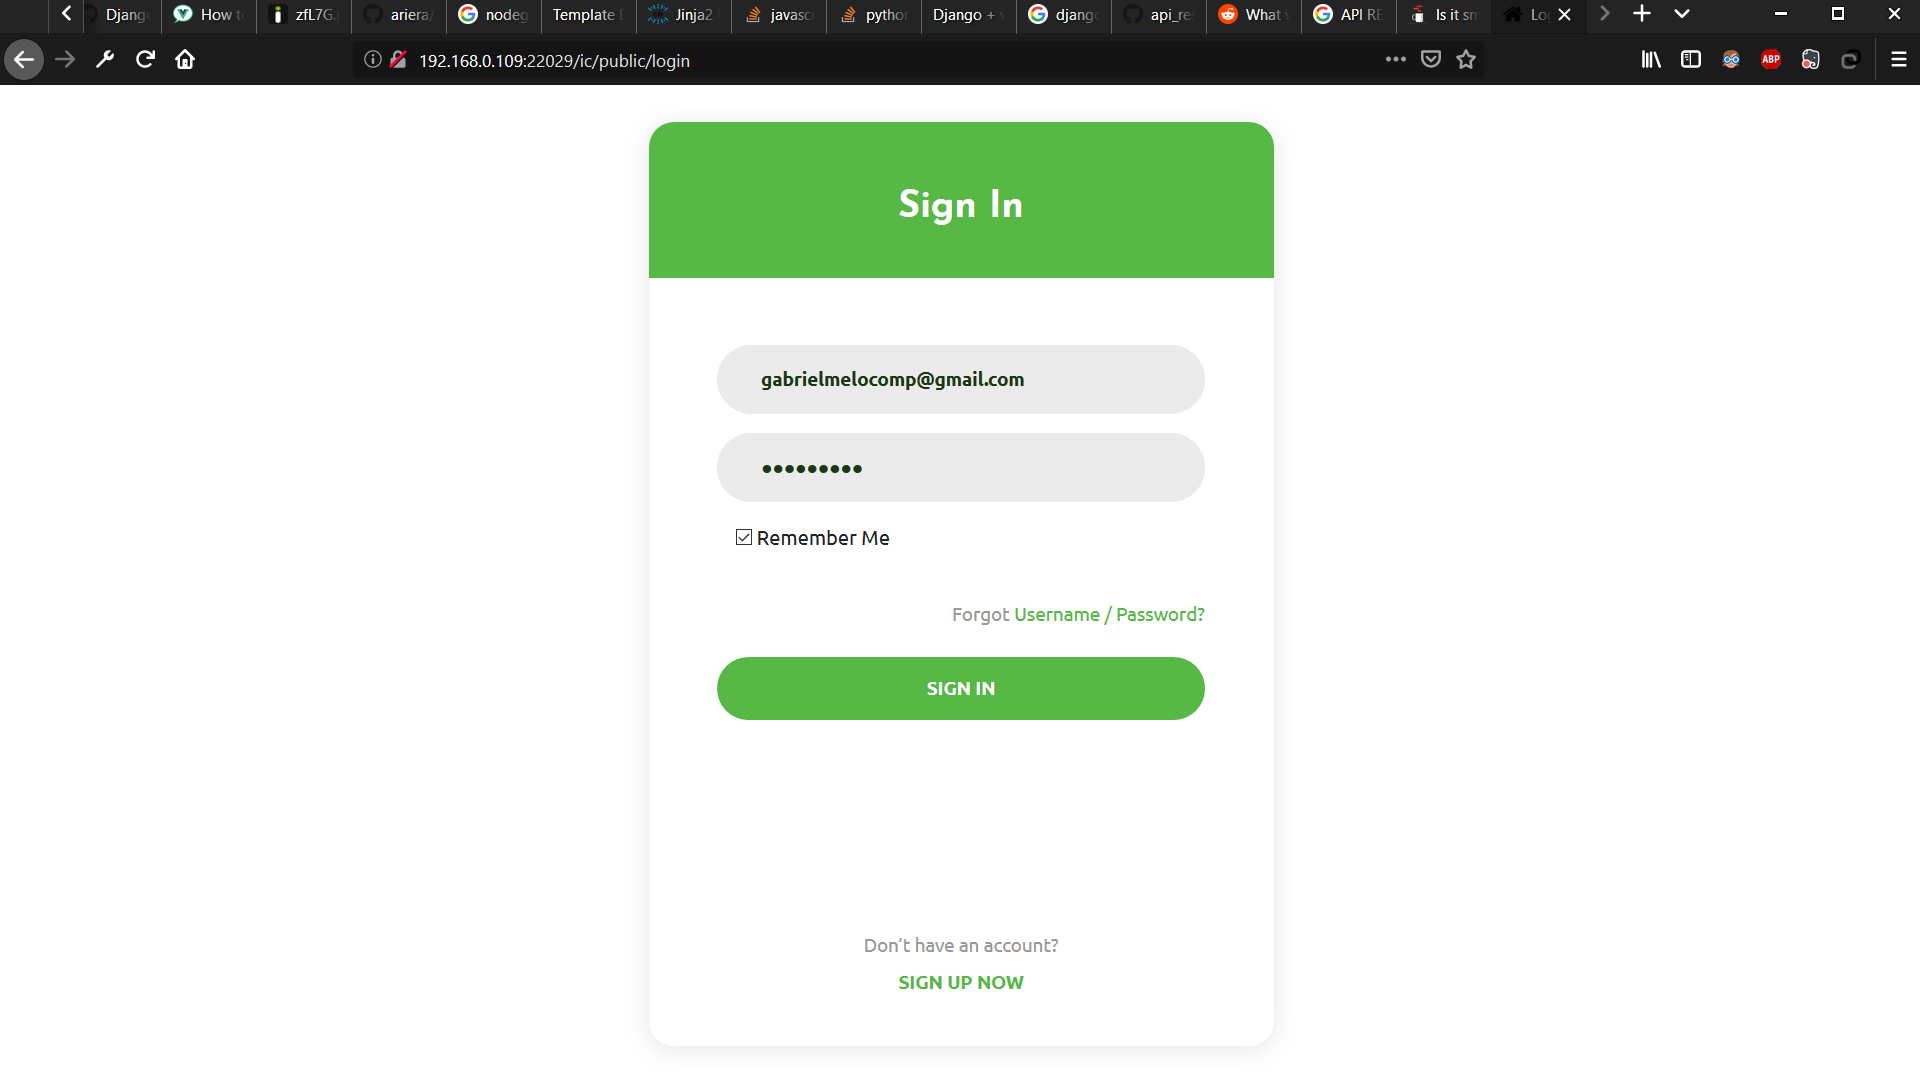
\includegraphics[width=300pt]{images/iot-server_login.png}
\end{frame}

\begin{frame}{Sistema de controle residencial}
  \frametitle{Sistema de controle residencial}
  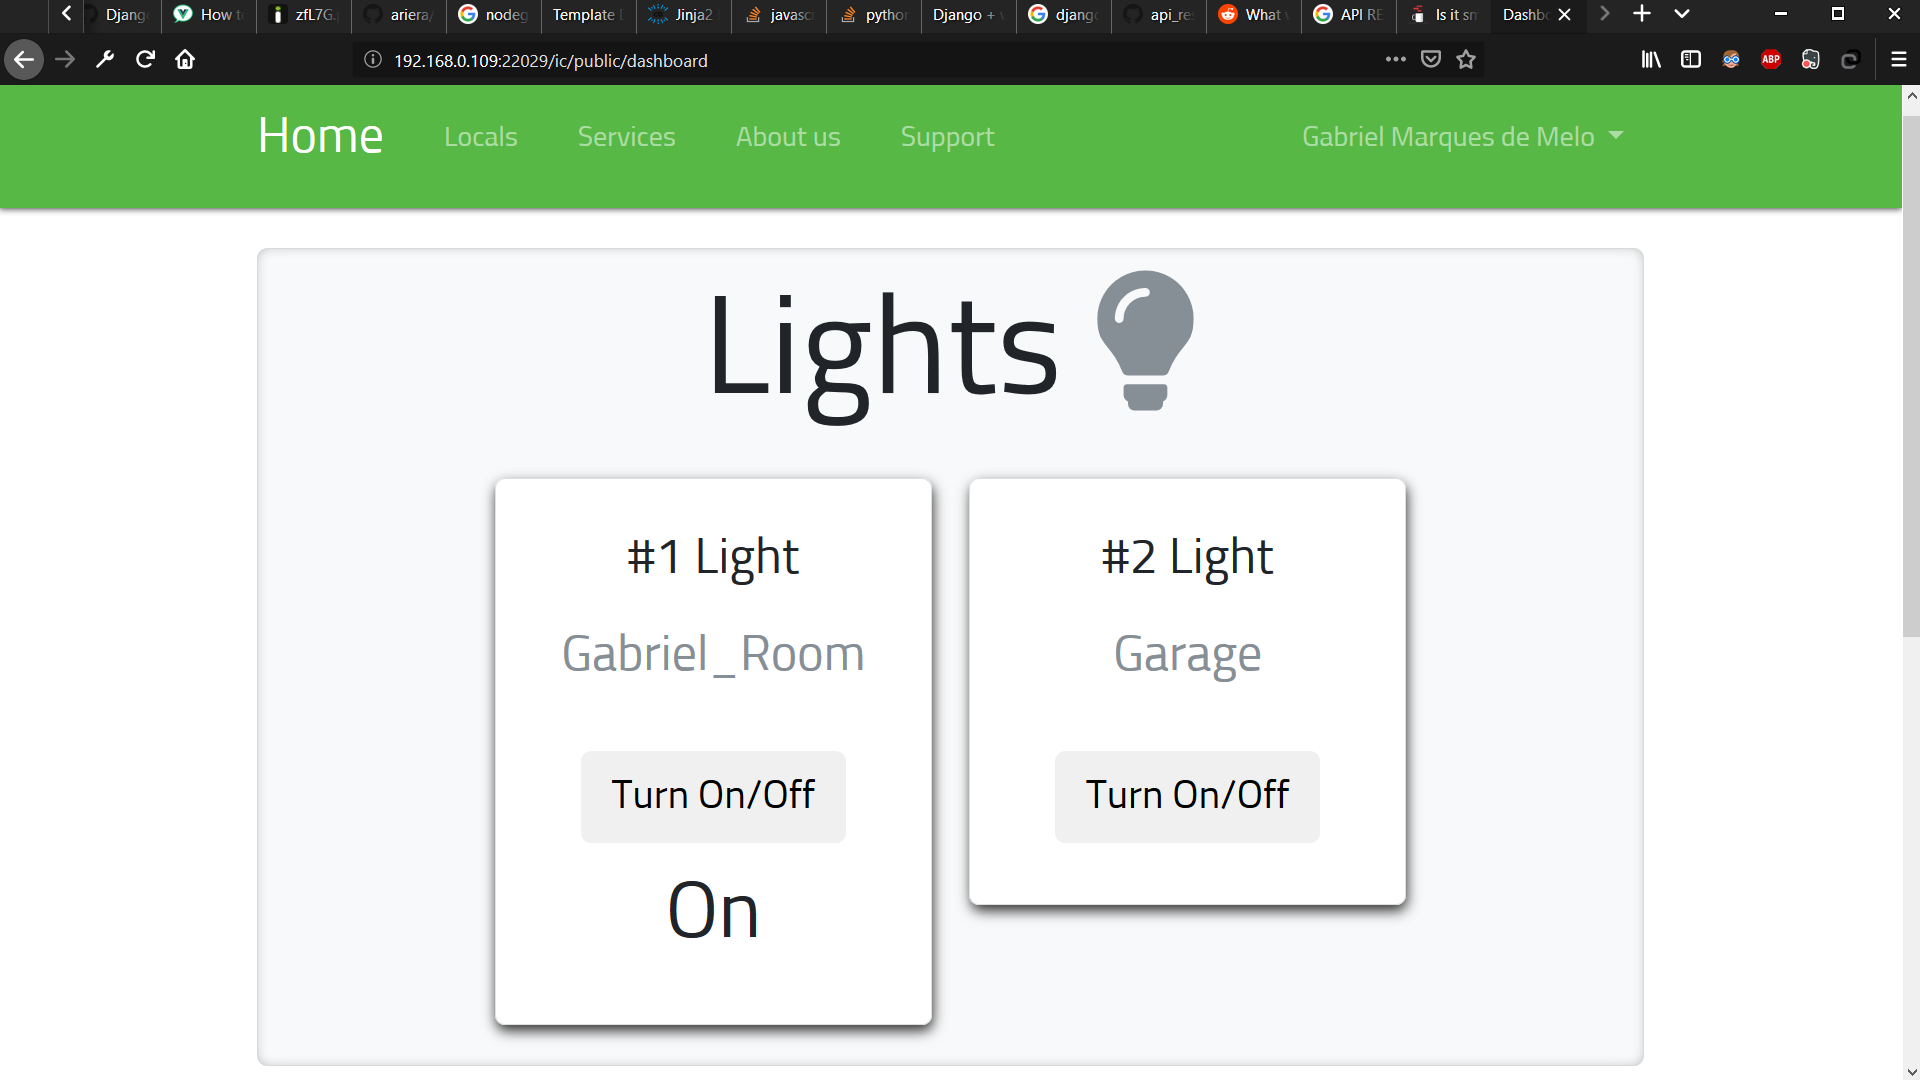
\includegraphics[width=300pt]{images/iot-server_dash1.png}
\end{frame}

\begin{frame}{Sistema de controle residencial}
  \frametitle{Sistema de controle residencial}
  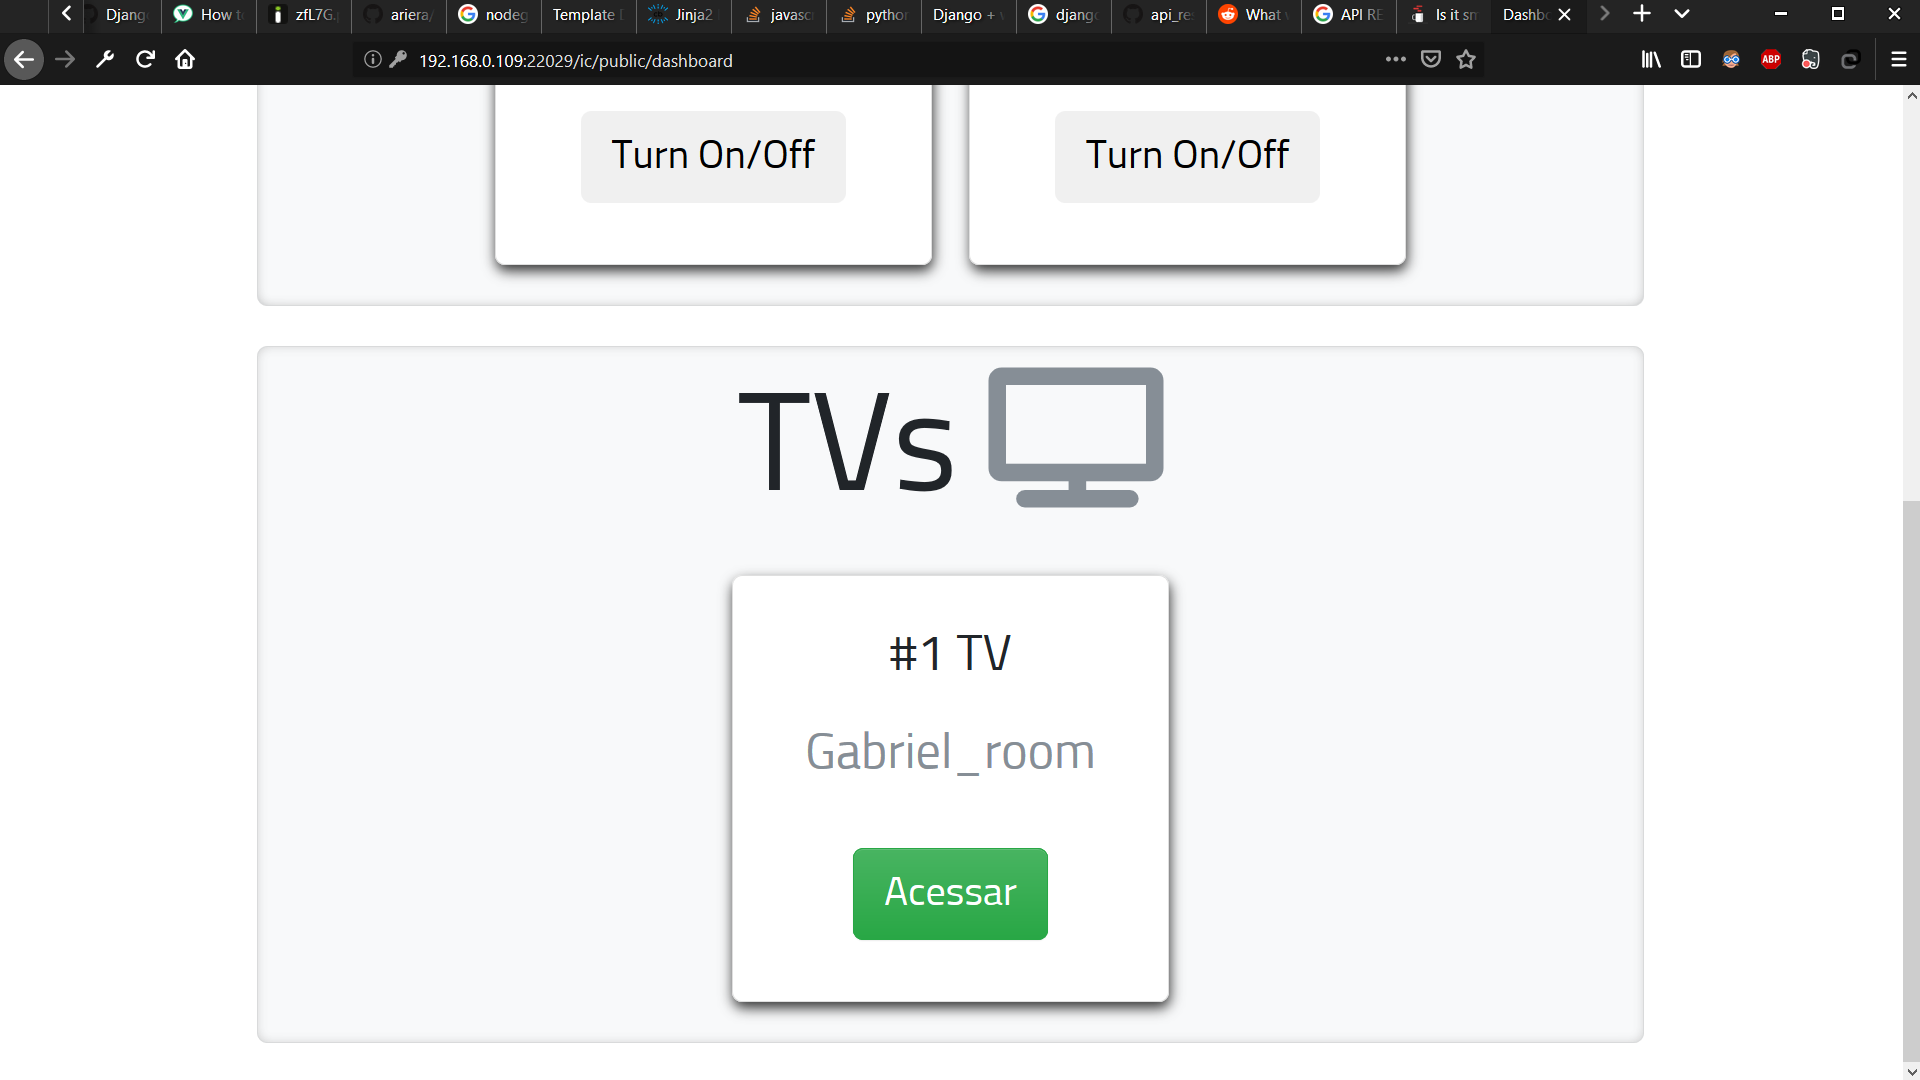
\includegraphics[width=300pt]{images/iot-server_dash2.png}
\end{frame}

\begin{frame}{Sistema de controle residencial}
  \frametitle{Sistema de controle residencial}
  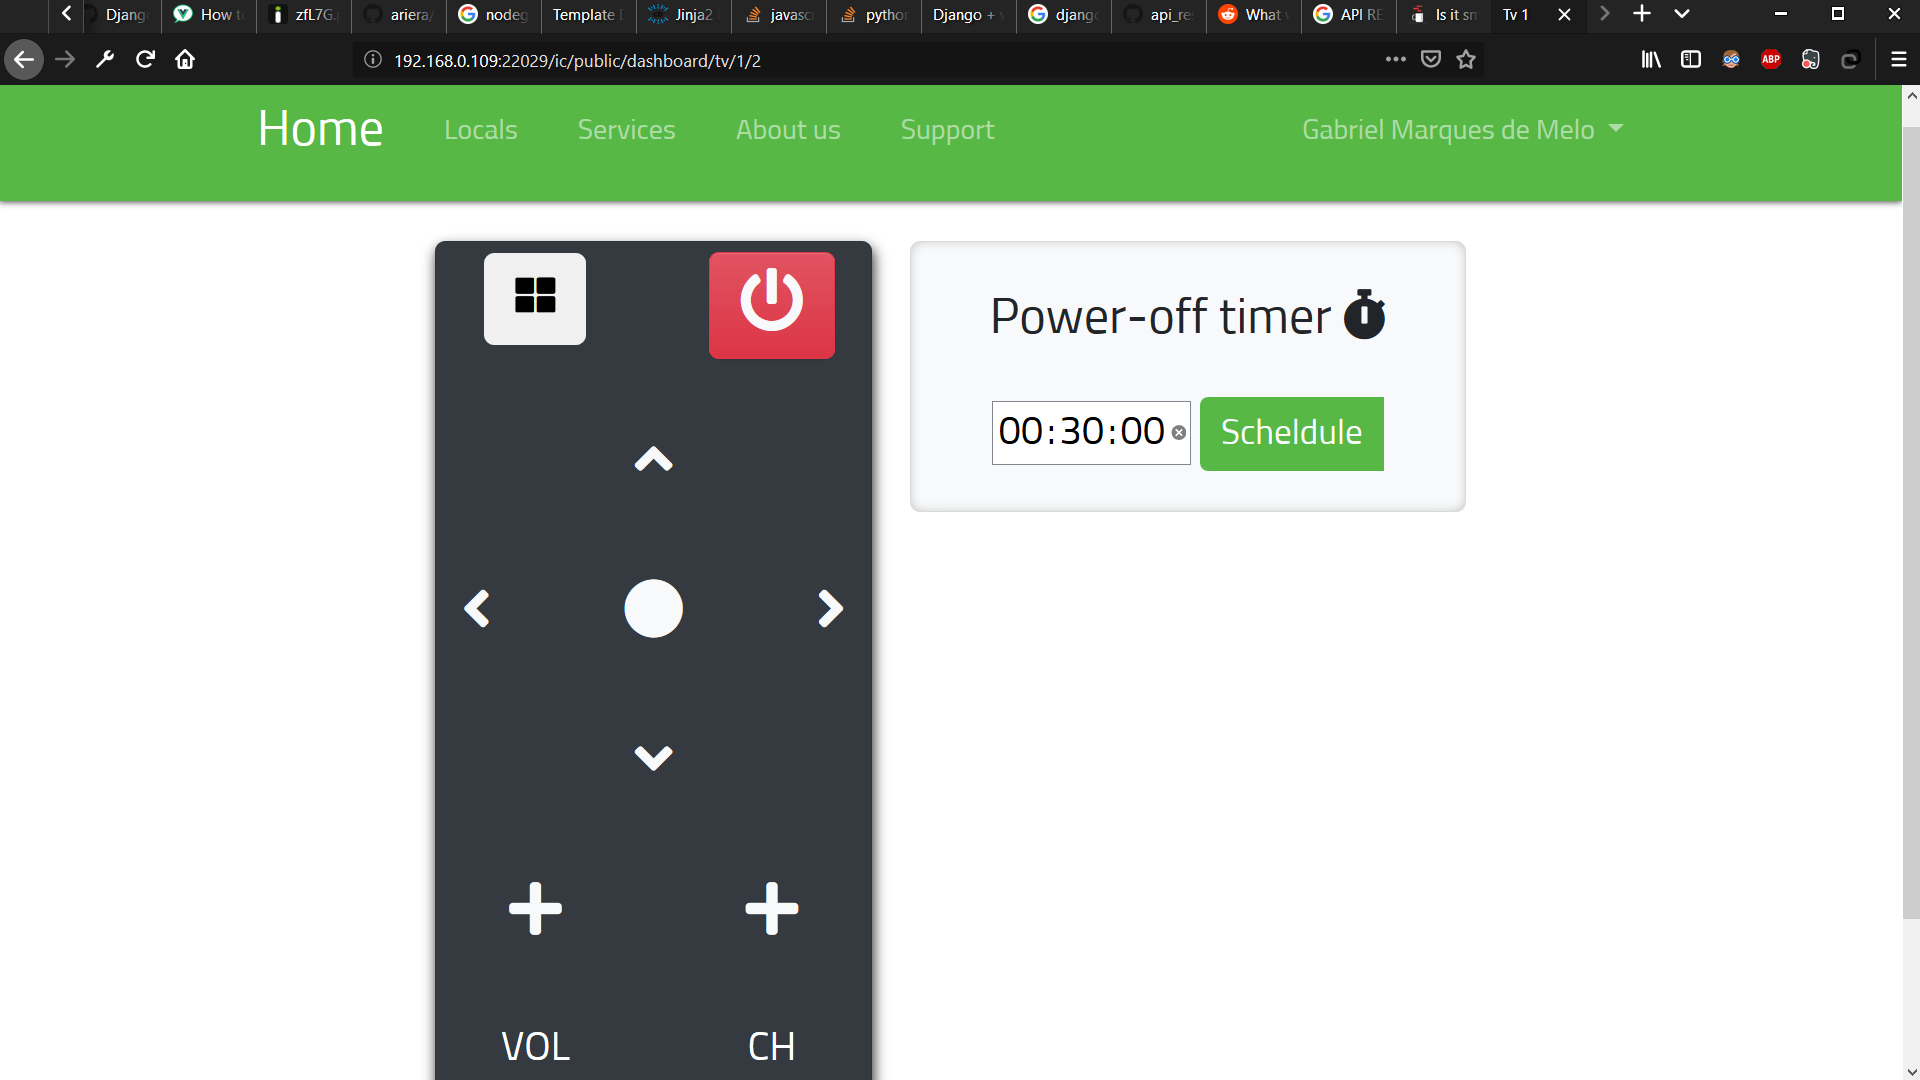
\includegraphics[width=300pt]{images/iot-server_remotecontrol.png}
\end{frame}
\section{Referências}

\begin{frame}{Summary}
  \frametitle{Referências}
  \begin{itemize}
    \item \textbf{Documentação Micropython}: https://docs.micropython.org/en/latest/esp8266/tutorial/intro.html \vspace{5pt}
    \item \textbf{Documentação Core Arduino/Esp8266}: https://docs.micropython.org/en/latest/esp8266/tutorial/intro.html \vspace{5pt}
    \item \textbf{ESP8266: Uma introdução ao IoT}, disponível em: https://github.com/GabrielMMelo/esp8266\_course
  \end{itemize}
\end{frame}

\plain{}{Perguntas?}

\end{document}
